%% abtex2-modelo-relatorio-tecnico.tex, v-1.8 laurocesar
%% Copyright 2012-2013 by abnTeX2 group at http://abntex2.googlecode.com/
%%
%% This work may be distributed and/or modified under the
%% conditions of the LaTeX Project Public License, either version 1.3
%% of this license or (at your option) any later version.
%% The latest version of this license is in
%%   http://www.latex-project.org/lppl.txt
%% and version 1.3 or later is part of all distributions of LaTeX
%% version 2005/12/01 or later.
%%
%% This work has the LPPL maintenance status `maintained'.
%%
%% The Current Maintainer of this work is the abnTeX2 team, led
%% by Lauro César Araujo. Further information are available on
%% http://abntex2.googlecode.com/
%%
%% This work consists of the files abntex2-modelo-relatorio-tecnico.tex,
%% abntex2-modelo-include-comandos and abntex2-modelo-references.bib
%%

% ------------------------------------------------------------------------
% ------------------------------------------------------------------------
% abnTeX2: Modelo de Relatório Técnico/Acadêmico em conformidade com
% ABNT NBR 10719:2011 Informação e documentação - Relatório técnico e/ou
% científico - Apresentação
% ------------------------------------------------------------------------
% ------------------------------------------------------------------------

\documentclass[
    % -- opções da classe memoir --
    12pt,				% tamanho da fonte
    openright,			% capítulos começam em pág ímpar (insere página vazia caso preciso)
    twoside,			% para impressão em verso e anverso. Oposto a oneside
    a4paper,			% tamanho do papel.
    % -- opções da classe abntex2 --
    %chapter=TITLE,		% títulos de capítulos convertidos em letras maiúsculas
    %section=TITLE,		% títulos de seções convertidos em letras maiúsculas
    %subsection=TITLE,	% títulos de subseções convertidos em letras maiúsculas
    %subsubsection=TITLE,% títulos de subsubseções convertidos em letras maiúsculas
    % -- opções do pacote babel --
    english,			% idioma adicional para hifenização
    french,				% idioma adicional para hifenização
    spanish,			% idioma adicional para hifenização
    brazil,				% o último idioma é o principal do documento
    ]{abntex2}


% ---
% PACOTES
% ---

% ---
% Pacotes fundamentais
% ---
\usepackage{cmap}				% Mapear caracteres especiais no PDF
\usepackage{lmodern}			% Usa a fonte Latin Modern
\usepackage[T1]{fontenc}		% Selecao de codigos de fonte.
\usepackage[utf8]{inputenc}		% Codificacao do documento (conversão automática dos acentos)
\usepackage{indentfirst}		% Indenta o primeiro parágrafo de cada seção.
\usepackage{color}				% Controle das cores
\usepackage{graphicx}			% Inclusão de gráficos
% ---

% ---
% Pacotes adicionais, usados no anexo do modelo de folha de identificação
% ---
\usepackage{multicol}
\usepackage{multirow}
% ---

% ---
% Pacotes adicionais, usados apenas no âmbito do Modelo Canônico do abnteX2
% ---
\usepackage{lipsum}				% para geração de dummy text
% ---

% ---
% Pacotes de citações
% ---
\usepackage[brazilian,hyperpageref]{backref}	 % Paginas com as citações na bibl
\usepackage[alf]{abntex2cite}	% Citações padrão ABNT

% ---
% CONFIGURAÇÕES DE PACOTES
% ---

% ---
% Configurações do pacote backref
% Usado sem a opção hyperpageref de backref
\renewcommand{\backrefpagesname}{Citado na(s) página(s):~}
% Texto padrão antes do número das páginas
\renewcommand{\backref}{}
% Define os textos da citação
\renewcommand*{\backrefalt}[4]{
    \ifcase #1 %
        Nenhuma citação no texto.%
    \or
        Citado na página #2.%
    \else
        Citado #1 vezes nas páginas #2.%
    \fi}%
% ---

% ---
% Informações de dados para CAPA e FOLHA DE ROSTO
% ---
\titulo{Projeto do\\ Sistema Gerenciador de Estágios\\ SIGEST}
\autor{Equipe LABENS}
\autor{Taciano de Morais Silva}
\local{Brasil}
\data{29/10/2013}
\instituicao{%
  Universidade Federal do Rio Grande do Norte -- UFRN
  \par
  Curso de Bacharelado em Sistemas de Informação
  \par
  DCEA/CERES}
\tipotrabalho{Relatório técnico}
% O preambulo deve conter o tipo do trabalho, o objetivo,
% o nome da instituição e a área de concentração
\preambulo{Minuta de Projeto do Sistema Gerenciador de Estágios do curso de Sistemas de Informação.}
% ---

% ---
% Configurações de aparência do PDF final

% alterando o aspecto da cor azul
\definecolor{blue}{RGB}{41,5,195}

% informações do PDF
\makeatletter
\hypersetup{
         %pagebackref=true,
        pdftitle={\@title},
        pdfauthor={\@author},
        pdfsubject={\imprimirpreambulo},
        pdfcreator={LaTeX with abnTeX2},
        pdfkeywords={abnt}{latex}{abntex}{abntex2}{relatório técnico},
        colorlinks=true,       		% false: boxed links; true: colored links
        linkcolor=blue,          	% color of internal links
        citecolor=blue,        		% color of links to bibliography
        filecolor=magenta,      		% color of file links
        urlcolor=blue,
        bookmarksdepth=4
}
\makeatother
% ---

% ---
% Espaçamentos entre linhas e parágrafos
% ---

% O tamanho do parágrafo é dado por:
\setlength{\parindent}{1.3cm}

% Controle do espaçamento entre um parágrafo e outro:
\setlength{\parskip}{0.2cm}  % tente também \onelineskip

% ---
% compila o indice
% ---
\makeindex
% ---

% ----
% Início do documento
% ----
\begin{document}

% Retira espaço extra obsoleto entre as frases.
\frenchspacing

% ----------------------------------------------------------
% ELEMENTOS PRÉ-TEXTUAIS
% ----------------------------------------------------------
% \pretextual

% ---
% Capa
% ---
\imprimircapa
% ---

% ---
% Folha de rosto
% (o * indica que haverá a ficha bibliográfica)
% ---
\imprimirfolhaderosto*
% ---

% ---
% Anverso da folha de rosto:
% ---

{
\ABNTEXchapterfont

\vspace*{\fill}

Conforme a ABNT NBR 10719:2011, seção 4.2.1.1.1, o anverso da folha de rosto
deve conter:

\begin{alineas}
  \item nome do órgão ou entidade responsável que solicitou ou gerou o
   relatório;
  \item título do projeto, programa ou plano que o relatório está relacionado;
  \item título do relatório;
  \item subtítulo, se houver, deve ser precedido de dois pontos, evidenciando a
   sua subordinação ao título. O relatório em vários volumes deve ter um título
   geral. Além deste, cada volume pode ter um título específico;
  \item número do volume, se houver mais de um, deve constar em cada folha de
   rosto a especificação do respectivo volume, em algarismo arábico;
  \item código de identificação, se houver, recomenda-se que seja formado
   pela sigla da instituição, indicação da categoria do relatório, data,
   indicação do assunto e número sequencial do relatório na série;
  \item classificação de segurança. Todos os órgãos, privados ou públicos, que
   desenvolvam pesquisa de interesse nacional de conteúdo sigiloso, devem
    informar a classificação adequada, conforme a legislação em vigor;
  \item nome do autor ou autor-entidade. O título e a qualificação ou a função
   do autor podem ser incluídos, pois servem para indicar sua autoridade no
   assunto. Caso a instituição que solicitou o relatório seja a mesma que o
   gerou, suprime-se o nome da instituição no campo de autoria;
  \item local (cidade) da instituição responsável e/ou solicitante; NOTA: No
   caso de cidades homônimas, recomenda-se o acréscimo da sigla da unidade da
   federação.
  \item ano de publicação, de acordo com o calendário universal (gregoriano),
  deve ser apresentado em algarismos arábicos.
\end{alineas}

\vspace*{\fill}
}
\cleardoublepage
% ---
% Agradecimentos
% ---
%\begin{agradecimentos}

%Agradecimentos!

%\end{agradecimentos}
% ---

% ---
% RESUMO
% ---

% resumo na língua vernácula (obrigatório)
\setlength{\absparsep}{18pt} % ajusta o espaçamento dos parágrafos do resumo
\begin{resumo}
 Segundo a \citeonline[3.1-3.2]{NBR6028:2003}, o resumo deve ressaltar o
 objetivo, o método, os resultados e as conclusões do documento. A ordem e a extensão
 destes itens dependem do tipo de resumo (informativo ou indicativo) e do
 tratamento que cada item recebe no documento original. O resumo deve ser
 precedido da referência do documento, com exceção do resumo inserido no
 próprio documento. (\ldots) As palavras-chave devem figurar logo abaixo do
 resumo, antecedidas da expressão Palavras-chave:, separadas entre si por
 ponto e finalizadas também por ponto.

 \noindent
 \textbf{Palavras-chaves}: latex. abntex. editoração de texto.
\end{resumo}
% ---

% ---
% inserir lista de ilustrações
% ---
\pdfbookmark[0]{\listfigurename}{lof}
\listoffigures*
\cleardoublepage
% ---

% ---
% inserir lista de tabelas
% ---
\pdfbookmark[0]{\listtablename}{lot}
\listoftables*
\cleardoublepage
% ---

% ---
% inserir lista de abreviaturas e siglas
% ---
\begin{siglas}
  \item[Fig.] Area of the $i^{th}$ component
  \item[456] Isto é um número
  \item[123] Isto é outro número
  \item[lauro cesar] este é o meu nome
\end{siglas}
% ---

% ---
% inserir lista de símbolos
% ---
\begin{simbolos}
  \item[$ \Gamma $] Letra grega Gama
  \item[$ \Lambda $] Lambda
  \item[$ \zeta $] Letra grega minúscula zeta
  \item[$ \in $] Pertence
\end{simbolos}
% ---

% ---
% inserir o sumario
% ---
\pdfbookmark[0]{\contentsname}{toc}
\tableofcontents*
\cleardoublepage
% ---


% ----------------------------------------------------------
% ELEMENTOS TEXTUAIS
% ----------------------------------------------------------
\textual

% ----------------------------------------------------------
% Introdução
% ----------------------------------------------------------
\chapter[Introdução]{Introdução}
%\addcontentsline{toc}{chapter}{Introdução}

Este documento e seu código-fonte são exemplos de referência de uso da classe
\textsf{abntex2} e do pacote \textsf{abntex2cite}. O documento
exemplifica a elaboração de relatórios técnicos e/ou científicos produzidos
conforme a ABNT NBR 10719:2011 \emph{Informação e documentação - Relatório
técnico e/ou científico - Apresentação}.

A expressão ``Modelo canônico'' é utilizada para indicar que \abnTeX\ não é
modelo específico de nenhuma universidade ou instituição, mas que implementa tão
somente os requisitos das normas da ABNT. Uma lista completa das normas
observadas pelo \abnTeX\ é apresentada em \citeonline{abntex2classe}.

Sinta-se convidado a participar do projeto \abnTeX! Acesse o site do projeto em
\url{http://abntex2.googlecode.com/}. Também fique livre para conhecer,
estudar, alterar e redistribuir o trabalho do \abnTeX, desde que os arquivos
modificados tenham seus nomes alterados e que os créditos sejam dados aos
autores originais, nos termos da ``The \LaTeX\ Project Public
License''\footnote{\url{http://www.latex-project.org/lppl.txt}}.

Encorajamos que sejam realizadas customizações específicas deste exemplo para
universidades e outras instituições --- como capas, folhas de rosto, etc.
Porém, recomendamos que ao invés de se alterar diretamente os arquivos do
\abnTeX, distribua-se arquivos com as respectivas customizações.
Isso permite que futuras versões do \abnTeX~não se tornem automaticamente
incompatíveis com as customizações promovidas. Consulte
\citeonline{abntex2-wiki-como-customizar} par mais informações.

Este documento deve ser utilizado como complemento dos manuais do \abnTeX\
\cite{abntex2classe,abntex2cite,abntex2cite-alf} e da classe \textsf{memoir}
\cite{memoir}.

Equipe \abnTeX

Lauro César Araujo


% ----------------------------------------------------------
% PARTE - preparação da pesquisa
% ----------------------------------------------------------
%\part{Preparação do relatório}

% ----------------------------------------------------------
% Capitulo com exemplos de comandos inseridos de arquivo externo
% ----------------------------------------------------------

\section{Lista de Requisitos}

O sistema gerenciador de estágios (SIGEST) deve antender os seguintes requisitos:

\begin{alineas}
  \item Manter cadastro de professores;
  \item Manter cadastro de empresas conveniadas;
  \item Manter cadastro de curso;
  \item Manter cadastro de estagiários;
  \item Manter cadastro de estágios;
	\item Manter cadastro de supervisores (funcionário das empresas conveniadas responsáveis diretos pelo estágio);
  \item Professores podem ser coordenadores de curso, coordenadores de estágio, orientadores de estágio, avaliadores de estágio;
  \item Manter o fluxo de andamento do estágio que pode estar nas seguintes situações: CADASTRADO PELO ALUNO, CADASTRADO PELO COORDENADOR,
	AGUARDANDO AUTORIZAÇÃO (que deve ser autorizado pelo COORDENADOR, SUPERVISOR e ORIENTADOR), AUTORIZADO, EM EXECUÇÃO, AGUARDANDO CADASTRO DE RELATÓRIO, EM AVALIAÇÃO, AGUARDANDO CORREÇÕES, APROVADO ou REPROVADO;
  \item Manter cadastro de atividades e cronograma do estágio;
  \item Gerar relatórios de acompanhamento mensais e semestrais;
	\item Manter calendário de datas importantes;
	\item Manter cadastro de e-mails de notícias e enviar e-mails automáticos para os interessados sempre que algo for atualizado no estágio.
\end{alineas}

Texto de introdução para testar a citação \cite{morais04a}.

\section{Definição de Perfis}

No sistema teremos vários tipos de usuário e seus respectivos perfis.
Segue abaixo a lista de usuários do sistema e seus respecitivos perfis.

\emph{Professor} - Entidade que representa o professor que pode assumir um dos
seguintes perfis:

\begin{itemize}
\item Coordenador de Curso
\item Coordenador Geral de Estágio
\item Avaliador de Estágio
\item Orientador de Estágio
\end{itemize}

Os perfis Avaliador e Orientador é organizado por estágios, podendo qualquer professor cadastrado ser avaliador de alguns estágios e 
orientador de alguns outros estágios. O orientador não avaliará os estágios que orienta. O coordenador de curso e o coordenador geral
de curso podem orientar e avaliar estágios. Os coordenadores são os únicos que podem cadastrar e alterar dados dos estágios.

\emph{Administrador} - Entidade que representa o super usuário que pode acessar e modificar
qualquer dado ou cadastro no sistema.

\chapter{Projeto Arquitetural}

\chapter{Modelo de Dados}

% Figura Modelo de Dados
\begin{figure}[!htb]
        \centering
        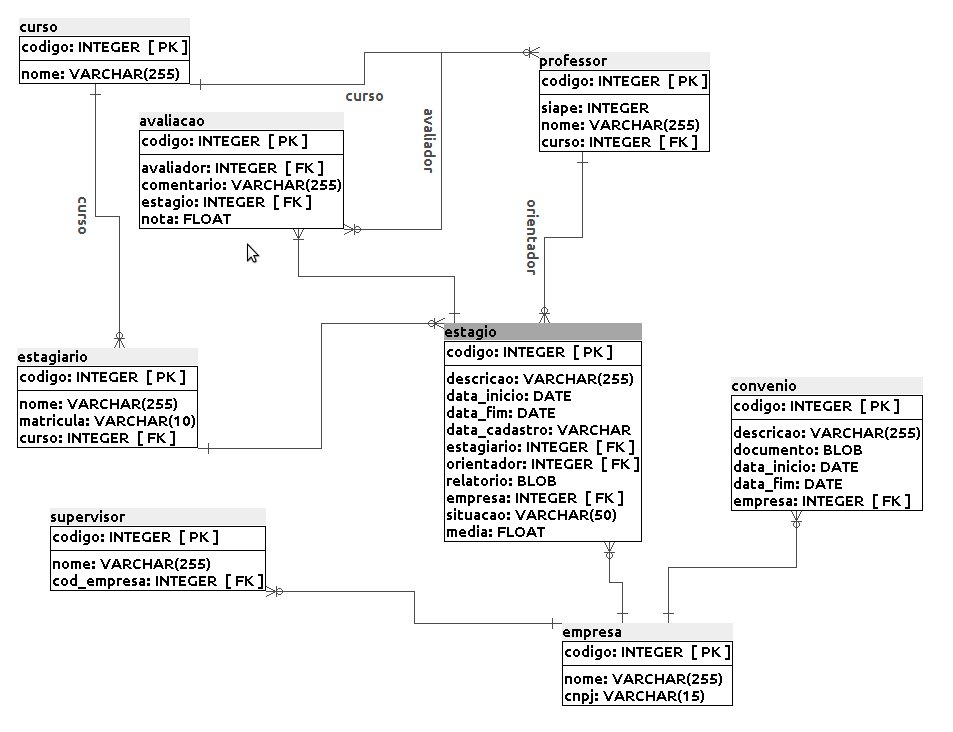
\includegraphics[scale=0.4]{esquema_sigest.jpg}
        \caption{Esquema Relacionado para o Sistema SIGEST}
        \label{fig:esquema_sigest}
\end{figure}
%\footnote{"A framework is a set of classes that embodies an abstract design for solutions to a family of related problems", \cite{johnson88}}


\chapter{Lista de Casos de Uso}

%% Input para a Section CDU001 - Estagiário
\section{CDU01 - Estagiário}

\subsection{Descrição}
A entidade Estagiário, será a responsável por conter as características e comportamentos que um estagiário real possui quando está pagando a disciplina Estágio.

Um estagiário real possui as seguintes características:

- Nome completo
- Matrícula
- Curso

Indiretamente, via entidade Estágio, ele será relacionado também as características que se seguem:

- Empresa vinculada
- Coordenador de estágio
- Orientador de estágio
- Supervisor de estágio
- Data de submissão de proposta
- Nota final


\subsection{Fluxo Principal}
O aluno que pretende se matricular na disciplina de Estágio, deve acessar o sistema e preencher todas informações referentes ao estágio em si e também suas informações pessoais, pois o
presente sistema não possui integração com o SIGAA para extrair informações acerca do aluno. Assim no fluxo principal é necessário que o aluno preencha suas informações pessoais como se segue.



\subsection{Fluxo Secundário}
Em segundo plano, a entidade Estágio será a responsável por ligar o Estagiário as demais informações do processo, como Empresa e Coordenador responsável por exemplo.
A ligação será feita no Banco de Dados via chaves extrangeiras, sempre obedecendo as normas formais.


\subsection{Fluxo de Exceção}

\subsection{Diagrama de Classe}

\subsection{Diagrama de Sequência}

\section{CDU02 - Estágio}

%\subsection{Descrição}
CDU002 - Estágio
    O estágio é o período em que um aluno trabalha para um empresa e realiza um
conjunto de atividades. As empresas podem receber alunos estagiários.
Cada estágio tem um professor orientador, um supervisor pertencente a empresa.

Um estagio possui os seguintes atributos:


Código do Estágio

Data Inicio

Data Final

Data de Cadastro do Aluno no estágio

Professor Orientador

Supervisor da Empresa

Empresa vinculada

Coordenador de estágio

Orientador de estágio

Supervisor de estágio

Nota final






\subsection{Fluxo Principal}


A resolver pois falta esclarecimentos sobre o projetos e documentação

\subsection{Fluxo Secundário}

A resolver pois falta esclarecimentos sobre o projetos e documentação

\subsection{Fluxo de Exceção}

\subsection{Diagrama de Classe}

\subsection{Diagrama de Sequência}

\section{CDU03 - Empresa}

%\subsection{Descrição}
CDU003 - Empresa
  A Entidade empresa será a instituição conveniada com a Universidade para receber estágiarios, no período em que ele esteja cursando a disciplina Estágio.

Uma Empresa possui os seguintes atributos:


+ Codigo da empresa

+ Cnpj

+ Nome

+ Descrição

+ Data do Convênio

\subsection{Fluxo Principal}

A resolver pois falta esclarecimentos sobre o projetos e documentação

\subsection{Fluxo Secundário}

A resolver pois falta esclarecimentos sobre o projetos e documentação

\subsection{Fluxo de Exceção}

\subsection{Diagrama de Classe}

\subsection{Diagrama de Sequência}

\section{CDU04 - Professor}

%\subsection{Descrição}

\subsection{Fluxo Principal}
1.  O sistema exibe o formulário para o cadastro de professor.
2.        O usuário preenche os campos de acordo com a RN001 e clica no botão cadastrar.
3.        O sistema persiste os dados. FE001
4.        O caso de uso termina.

\subsection{Fluxo Secundário}
FE001 - Se houver algum erro ao persistir os dados, o sistema exibe a mensagem  MSG001 e retorna ao passo 2 com os dados já preenchidos. Se não o sistema exibe a mensagem MSG002 e continua com o passo seguinte.

\subsection{Regra de Negócio}
    RN001 - Todos os campos em negrito são obrigatórios.

\subsection{Mensagens do Sistema}
    MSG001 - “Erro ao salvar dados.”
    MSG002 - “Professor cadastrado com sucesso!”

\subsection{Fluxo de Exceção}

\subsection{Diagrama de Classe}

\subsection{Diagrama de Sequência}

\section{CDU005 - Curso}

%\subsection{Descrição}
A entidade \emph{Curso}, será a responsável por representar e armazenar as
características de um curso que receberá alunos para estágios.

Um \emph{Curso} possui as seguintes características:

\begin{itemize}
  \item código: Numérico tipo serial;
  \item nome: Texto tipo varchar;
  \item coordenador: Numérico tipo serial - código de um professor;
  \item vice coordenador: Numérico tipo serial - código de um professor;
  \item coordenador de estágios: Numérico tipo serial - código de um professor;
  \item resolução de estágios: Binário - tipo  blob para enviar um pdf;
  \item fórmulários avaliativos para os estágios (voluntários ou obrigatórios);
\end{itemize}

A entidade Curso terá relacionamentos com as seguintes entidades:

\begin{itemize}
  \item Estágios de alunos do curso;
  \item Coordenador do curso - um professor;
  \item Vice coordenador do curso - um professor;
  \item Coordenador de estágios - um professor;
\end{itemize}

\subsection{Fluxo Principal}

Dependendo dos atores a entidade curso poderá ser acessada de formas diferentes.
Temos os seguintes atores possíveis: Professor, Coordenador, Aluno Estagiário e
Supervisor.

\subsubsection{Incluir Curso}

Para incluir um curso o ator segue os seguintes passos:

\begin{itemize}
  \item O ator faz login no sistema;
  \item O sistema verifica se o ator tem permissão para a função (apenas
  administradores);
  \item O sistema abre a tela para cadastrar um novo curso;
  \item O ator preenche os dados do curso;
  \item O ator salva o novo curso;
\end{itemize}


\subsubsection{Alterar Curso}

\begin{itemize}
  \item O ator faz login no sistema;
  \item O sistema verifica se o ator tem permissão para a função (apenas
  administradores);
  \item O sistema abre a tela para alterar o curso;
  \item O ator preenche os dados do curso;
  \item O ator salva as alterações curso;
\end{itemize}

\subsubsection{Consultar Curso}

\begin{itemize}
  \item O ator faz login no sistema;
  \item O sistema verifica se o ator tem permissão para a função (apenas
  administradores);
  \item O sistema abre a tela para consultar e listar os cursos;
\end{itemize}

\subsection{Fluxo Secundário}

\subsubsection{Consultar Estágios do Curso}

\begin{itemize}
  \item O ator faz login no sistema;
  \item O sistema verifica se o ator tem permissão para a função;
  \item O sistema abre a tela para consultar e listar os cursos;
  \item O ator define as informações de filtragem;
  \item O sistema apresenta a lista de estágios do curso;
\end{itemize}

\subsection{Fluxo de Exceção}

\subsection{Diagrama de Classe}

\subsection{Diagrama de Sequência}

% ---
% Finaliza a parte no bookmark do PDF, para que se inicie o bookmark na raiz
% ---
\bookmarksetup{startatroot}%
% ---

% ---
% Conclusão
% ---
\chapter*[Conclusão]{Conclusão}
\addcontentsline{toc}{chapter}{Conclusão}

\lipsum[31-33]

% ----------------------------------------------------------
% ELEMENTOS PÓS-TEXTUAIS
% ----------------------------------------------------------
\postextual

% ----------------------------------------------------------
% Referências bibliográficas
% ----------------------------------------------------------

%%%%%%%%%%%%%%%%%%%%%%%%%%%%%%%%%%%%%%%%%%%%%%%%%%%%%%%%%%%%%%%%%%%%%%%%%%%%%%%
%% Bibliografia

%\bibliographystyle{alpha} % estilo de bibliografia
\bibliography{bibliografia} % arquivos com as entradas bib.

%%%%%%%%%%%%%%%%%%%%%%%%%%%%%%%%%%%%%%%%%%%%%%%%%%%%%%%%%%%%%%%%%%%%%%%%%%%%%%%
%% Ap\^endice
% Caso seja necessário algum apêndice!

\end{document}